\documentclass[11pt]{article}
\newcommand{\coursedocname}{Problem Set 1}

\usepackage[utf8]{inputenc}
\usepackage[T1]{fontenc}
\usepackage{lmodern}
\usepackage[margin=1in]{geometry}
\usepackage[dvipsnames]{xcolor}
\usepackage{graphicx, booktabs, enumitem, float, framed, caption, multirow}
\usepackage{fancyhdr}
\usepackage{tcolorbox}
\usepackage{listings}
\usepackage{tikz}
\usepackage{setspace}
\usepackage{needspace}
\IfFileExists{algorithm.sty}{%
  \usepackage{algorithm}
  \usepackage[noend]{algpseudocode}
  \newcommand{\hasalgorithms}{}%
}{}
\usepackage{amsmath,amssymb,bm,xcolor}



\newcommand{\disc}{\gamma}              %
\newcommand{\Vfun}{V}                   %
\newcommand{\heur}{h}                   %
\newcommand{\ctg}{g}                    %



\usepackage{hyperref}

\definecolor{DartmouthGreen}{HTML}{00693E}
\newcommand{\dgreen}[1]{\textcolor{DartmouthGreen}{#1}}
\newcommand{\dgbf}[1]{\textbf{\dgreen{#1}}}      %
\urlstyle{same}
\hypersetup{
    colorlinks=true,
    linkcolor=DartmouthGreen,
    filecolor=DartmouthGreen,
    citecolor=DartmouthGreen,
    urlcolor=DartmouthGreen,
    breaklinks=true
}

\newcommand{\coursenumber}{COSC 81/281}
\newcommand{\courseterm}{Fall 2026}
\newcommand{\gradescopelink}{\textbf{Gradescope} (\url{https://www.gradescope.com/courses/1372528})}

\newcommand{\psOneDue}{Tuesday, September 29 (11:59pm ET)}

\setlength{\parindent}{0pt}
\setlength{\parskip}{6pt plus 2pt minus 1pt}
\setlength{\headheight}{13.6pt}
\setlength{\emergencystretch}{3em}
\setcounter{secnumdepth}{0}

\DeclareRobustCommand{\callout}[2][gray!10]{%
  \begin{tcolorbox}[left=8pt, arc=0pt, outer arc=0pt,
                    colframe=#1, colback=#1, coltext=black]#2\end{tcolorbox}}




\newcommand{\gradstar}{$\bigstar$~\textsf{\small (required for 281; optional for 81)}~}
\newcommand{\bonusq}{\textsf{\small\textbf{[Bonus]}}~}
\newcommand{\bonus}{\bonusq}

\newcommand{\setupheader}[1]{%
  \fancypagestyle{default}{%
      \lhead{#1}
      \chead{}
      \rhead{\textbf{\coursenumber}}
      \lfoot{}
      \cfoot{}
      \rfoot{\thepage}
      \renewcommand{\headrulewidth}{0.4pt}
      \renewcommand{\footrulewidth}{0.4pt}
  }
  \pagestyle{default}
  \fancypagestyle{plain}{\pagestyle{default}}
}
\newcommand{\setupexamheader}[1]{%
  \fancypagestyle{default}{%
      \lhead{#1}
      \chead{Name:}
      \rhead{}
      \lfoot{}
      \cfoot{}
      \rfoot{\thepage}
      \renewcommand{\headrulewidth}{0.4pt}
      \renewcommand{\footrulewidth}{0.4pt}
  }
  \pagestyle{default}
  \fancypagestyle{plain}{\pagestyle{default}}
}
\newcommand{\pstitle}[2]{%
  \title{\textbf{\coursenumber:} #1}
  \author{\textbf{Due} #2\\
  }
  \date{}
}

\newcommand{\coursenotice}{%
  \callout{Problem sets are graded \textbf{pass/fail on completion}, and
  there are no late days. The problem sets are where the learning happens,
  and they are the best available practice for the midterm and final exam.
  Submit to \gradescopelink\ and assign each question to a page in your
  submission. Questions are welcome on \dgbf{Slack}. Starred ($\bigstar$)
  questions are required for COSC 281 students and optional (ungraded) for
  COSC 81 students.}}

\lstset{
  language=python,
  basicstyle=\ttfamily,
  commentstyle=\color{BrickRed},
  stringstyle=\color{ForestGreen},
  showstringspaces=false,
  breaklines=true,
  breakatwhitespace=true,
  keywordstyle=\color{Purple},
  emph={def},
  emphstyle=\color{RoyalBlue}
}
\lstnewenvironment{itemlisting}[1][]
 {\mbox{}\vspace*{-\baselineskip}%
  \lstset{xleftmargin=\leftmargin, linewidth=\linewidth, #1}}
 {}

\makeatletter
\def\fps@figure{htbp}
\makeatother
\ifdefined\hasalgorithms
\fi

\newcommand{\docfooter}{\vfill\begin{tiny}Updated \today\end{tiny}}


\newenvironment{studentanswer}[1]
  {\par\medskip\noindent
   \begin{tcolorbox}[height from=#1 to 100cm, colback=white, colframe=gray!60,
     boxrule=0.6pt, arc=0pt, outer arc=0pt, left=7pt, right=7pt,
     top=7pt, bottom=7pt, title={Answer / work}, fonttitle=\small,
     coltitle=black, colbacktitle=gray!8, titlerule=0pt]
   \ignorespaces}
  {\end{tcolorbox}\par}


\setupheader{\coursenumber\ -- \courseterm\ -- \coursedocname}
\pstitle{Problem Set 1: Search, Values, and Sampling}{\psOneDue}

\begin{document}
\maketitle
\coursenotice
\begin{quote}\small\textbf{AI Policy.} You may use any AI tools you like to assist you with your assignments, and you should, as that is likely how you will work for the rest of your career. 
That being said, the written portions are practice for the in-class midterm and exam, which are closed book and on paper. You should strive to answer these yourself and use AI as a tutor and not an oracle.
\end{quote}

\callout{Please include an AI Tool Disclosure Below \vspace{50pt}}

\raggedbottom
\section{Overview}

This problem set examines three approaches to robot motion planning:
search, value-based methods, and sampling. You will implement A* to find
shortest paths on a grid, value iteration and policy iteration to compute
policies for a grid-based Markov decision process (MDP), and a
Rapidly-exploring Random Tree (RRT) to plan motions for a car with a
minimum turning radius. By comparing these methods on the same maps,
you will examine how the state representation and computational cost
affect the resulting plans. The written problems provide practice with the calculations, proofs, and
reasoning expected on exams.

\clearpage
\textbf{Getting the code.} Pull the course repository. The starter code
is in \texttt{ps1/code/}, and the three maps, \texttt{open},
\texttt{maze}, and \texttt{narrow}, are in \texttt{sim/maps/}. The starter
provides the search frontier, grid MDP, car motion primitives, collision
checks, and plotting functions. Your implementations belong in
\texttt{astar.py}, \texttt{vi.py}, \texttt{policy\_iteration.py}, and
\texttt{rrt.py}.

\callout{\textbf{A* tie-breaking convention.} Expand the frontier node
with the smallest $f = \ctg + \heur$. If multiple nodes have the same
$f$-value, choose the node with the smallest $\heur$. If these values
are also equal, choose the smallest row index, followed by the smallest
column index. Row and column indices begin at 0 in the top-left corner.
Use this convention for both the written problems and the programming
task; the provided \texttt{DeterministicFrontier} implements it.}

\textbf{What to submit.} Submit the following to \gradescopelink:
\begin{enumerate}
\item \textbf{Written work (PDF):} Include your answers to Part 1 and the
      tables, figures, and explanations requested in Part 2. You may
      write in the answer boxes, annotate the PDF, or prepare a separate
      document. To use \texttt{ps1/handout.tex}, enter your responses below
      the \texttt{\%\%\%\%\% SOLUTION HERE \%\%\%\%\%} markers in the
      corresponding \texttt{studentanswer} environments and compile the
      file. The boxes expand to accommodate typed responses. You may add
      pages for figures or longer answers. Assign each question to its
      corresponding page or pages when uploading.
\item \textbf{Code:} Submit \texttt{astar.py}, \texttt{vi.py},
      \texttt{policy\_iteration.py}, and \texttt{rrt.py}. Before submitting,
      run \texttt{python ps1/code/autograder.py} from the repository root.
\end{enumerate}

\clearpage
\section{Part 1: Written problems}

These problems provide practice for the types of questions asked on
exams. Show your work. Numerical answers can be expressed as small
integers or simple fractions, so a calculator is not required.

\subsection*{P1: A*}

The grid below is 4-connected with unit step cost. Dark cells are obstacles.
You start at $S = (0,0)$ with goal $G = (3,3)$. Coordinates are given as
(row, column), with $S$ in the top-left corner. Use Manhattan distance to
$G$ as the heuristic; its value is printed in each open cell other than
the goal, where it is zero. Break ties in $f$ using the smaller heuristic
value, then the smaller row index, and finally the smaller column index.
\begin{center}
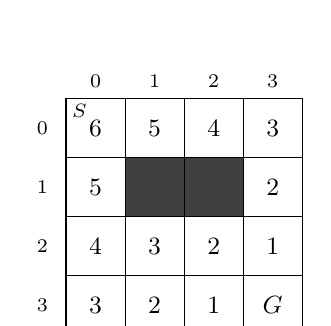
\begin{tikzpicture}[scale=0.75, every node/.style={font=\small}]
  \fill[black!75] (1,-2) rectangle (3,-1);
  \draw[step=1] (0,-4) grid (4,0);
  \foreach \c in {0,1,2,3} \node at (\c+0.5, 0.3) {\scriptsize \c};
  \foreach \r in {0,1,2,3} \node at (-0.4, -\r-0.5) {\scriptsize \r};
  \node[anchor=north west, inner sep=2pt] at (0,0) {\scriptsize$S$};
  \node at (0.5,-0.5) {$6$};
  \node at (1.5,-0.5) {$5$};
  \node at (2.5,-0.5) {$4$};
  \node at (3.5,-0.5) {$3$};
  \node at (0.5,-1.5) {$5$};
  \node at (3.5,-1.5) {$2$};
  \node at (0.5,-2.5) {$4$};
  \node at (1.5,-2.5) {$3$};
  \node at (2.5,-2.5) {$2$};
  \node at (3.5,-2.5) {$1$};
  \node at (0.5,-3.5) {$3$};
  \node at (1.5,-3.5) {$2$};
  \node at (2.5,-3.5) {$1$};
  \node at (3.5,-3.5) {$G$};
\end{tikzpicture}
\end{center}

\begin{enumerate}[label=(\alph*)]

\Needspace{3.9cm}
\item List the first \textbf{five} nodes that A* expands, in order, and give the $f$-value of each node at expansion. For each tie, identify the rule that determines which node is expanded.

\begin{studentanswer}{2.5cm}
%%%%% SOLUTION HERE %%%%%
\end{studentanswer}

\Needspace{3.0cm}
\item State the cost of the path returned by A* and write out one optimal path.

\begin{studentanswer}{1.6cm}
%%%%% SOLUTION HERE %%%%%
\end{studentanswer}

\Needspace{3.4cm}
\item The node $(1,0)$ is on the frontier with $f=6$ after the first expansion, but A* reaches the goal without expanding it. Explain in two sentences how the tie-breaking rules produce this result.

\begin{studentanswer}{2.0cm}
%%%%% SOLUTION HERE %%%%%
\end{studentanswer}

\end{enumerate}

\clearpage
\subsection*{P2: Heuristic admissibility}

Consider the following heuristics for a cell $n$ and goal $G$ on a
4-connected unit-cost grid with obstacles. Let $\Delta r = |r_n-r_G|$
and $\Delta c = |c_n-c_G|$:
\[
\heur_A(n)=\max(\Delta r,\Delta c), \qquad
\heur_B(n)=\Delta r+\Delta c+2N_{\mathrm{obs}},
\]
where $N_{\mathrm{obs}}$ counts the obstacle cells in the axis-aligned
rectangle whose opposite corners are $n$ and $G$, including its boundary.
The additional term in $\heur_B$ is intended to account for detours
around obstacles. In the grid below, $G=(0,2)$ and the only obstacle is
at $(1,1)$.
\begin{center}
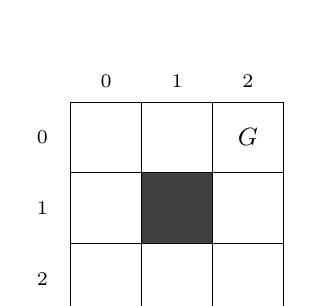
\begin{tikzpicture}[scale=0.9, every node/.style={font=\small}]
  \fill[black!75] (1,-2) rectangle (2,-1);
  \draw[step=1] (0,-3) grid (3,0);
  \foreach \c in {0,1,2} \node at (\c+0.5, 0.3) {\scriptsize \c};
  \foreach \r in {0,1,2} \node at (-0.4, -\r-0.5) {\scriptsize \r};
  \node at (2.5,-0.5) {$G$};
\end{tikzpicture}
\end{center}

\begin{enumerate}[label=(\alph*)]

\Needspace{3.6cm}
\item State the definition of an admissible heuristic.

\begin{studentanswer}{1.8cm}
%%%%% SOLUTION HERE %%%%%
\end{studentanswer}

\Needspace{4.8cm}
\item Prove in two or three sentences that $\heur_A$ is admissible on every 4-connected unit-cost grid, including grids with obstacles.

\begin{studentanswer}{3cm}
%%%%% SOLUTION HERE %%%%%
\end{studentanswer}

\Needspace{5.8cm}
\item Determine whether $\heur_B$ is admissible. If it is, provide a proof. If it is not, identify a cell in the grid above, compute both $\heur_B$ and the optimal cost-to-go at that cell, and explain why counting obstacles does not give a valid lower bound.

\begin{studentanswer}{4cm}
%%%%% SOLUTION HERE %%%%%
\end{studentanswer}

\end{enumerate}

\clearpage
\subsection*{P3: Value iteration}

The $4\times4$ grid below uses (row, column) coordinates, with row 0 at
the top and column 0 at the left. Dark cells are walls. Actions move
deterministically north, south, east, or west. An action that would cross
a wall or grid boundary leaves the robot in its current cell. Entering
the goal $G=(0,3)$ gives reward $+4$ and ends the episode; all other
transitions give reward 0. Set $\Vfun(G)=0$, use discount factor
$\disc=\tfrac12$, and initialize $\Vfun_0=0$ at every cell. A synchronous
sweep computes all entries of $\Vfun_{k+1}$ using only $\Vfun_k$.
\begin{center}
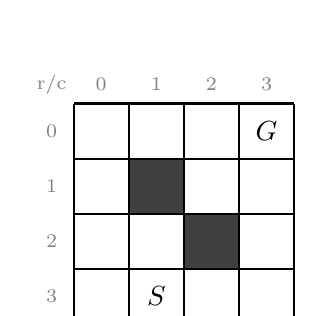
\begin{tikzpicture}[scale=0.7]
\fill[black!75] (1,2) rectangle (2,3);   %
\fill[black!75] (2,1) rectangle (3,2);   %
\draw[step=1, thick] (0,0) grid (4,4);
\node at (3.5,3.5) {$G$};
\node at (1.5,0.5) {$S$};
\foreach \r in {0,1,2,3} \node[font=\scriptsize, gray] at (-0.4, 3.5-\r) {\r};
\foreach \c in {0,1,2,3} \node[font=\scriptsize, gray] at (\c+0.5, 4.35) {\c};
\node[font=\scriptsize, gray] at (-0.4, 4.35) {r/c};
\end{tikzpicture}
\end{center}

\begin{enumerate}[label=(\alph*)]

\Needspace{5.5cm}
\item Perform one synchronous sweep. Use the grid provided to enter $\Vfun_1$ at every free cell.

\begin{studentanswer}{4cm}
%%%%% SOLUTION HERE %%%%%
\begin{center}
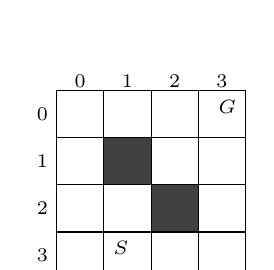
\begin{tikzpicture}[scale=0.6]
\fill[black!75] (1,2) rectangle (2,3);
\fill[black!75] (2,1) rectangle (3,2);
\draw[step=1] (0,0) grid (4,4);
\node[anchor=north east,font=\scriptsize] at (4,4) {$G$};
\node[anchor=north west,font=\scriptsize] at (1,1) {$S$};
\foreach \r in {0,1,2,3} \node[font=\scriptsize] at (-0.3,3.5-\r) {\r};
\foreach \c in {0,1,2,3} \node[font=\scriptsize] at (\c+0.5,4.2) {\c};
\end{tikzpicture}
\end{center}
\end{studentanswer}

\item Perform a second synchronous sweep. Use the grid provided to enter $\Vfun_2$ at every free cell.

\begin{studentanswer}{4cm}
%%%%% SOLUTION HERE %%%%%
\begin{center}
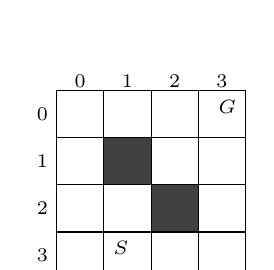
\begin{tikzpicture}[scale=0.6]
\fill[black!75] (1,2) rectangle (2,3);
\fill[black!75] (2,1) rectangle (3,2);
\draw[step=1] (0,0) grid (4,4);
\node[anchor=north east,font=\scriptsize] at (4,4) {$G$};
\node[anchor=north west,font=\scriptsize] at (1,1) {$S$};
\foreach \r in {0,1,2,3} \node[font=\scriptsize] at (-0.3,3.5-\r) {\r};
\foreach \c in {0,1,2,3} \node[font=\scriptsize] at (\c+0.5,4.2) {\c};
\end{tikzpicture}
\end{center}
\end{studentanswer}

\Needspace{3.9cm}
\item \gradstar For the start $S=(3,1)$, identify the first sweep at which $\Vfun_k(S)\neq0$ and compute its value. Explain how the shortest-path distance allows you to answer without performing each intermediate sweep.

\begin{studentanswer}{2.5cm}
%%%%% SOLUTION HERE %%%%%
\end{studentanswer}

\end{enumerate}

\clearpage
\subsection*{P4: Admissibility and consistency on a graph}

Consider the directed graph below, with start $S$, goal $G$, and positive
edge costs. Only the arrows shown are available. For every heuristic,
assume $h(G)=0$ and nonnegative values. Admissibility requires
$h(n)\leq h^*(n)$ at every node, where $h^*(n)$ is the least cost to the
goal. Consistency additionally requires $h(u)\leq c(u,v)+h(v)$ for every
directed edge $u\to v$.

\begin{center}
\begin{minipage}[c]{0.48\linewidth}\centering
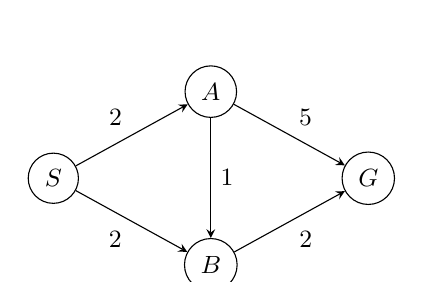
\begin{tikzpicture}[>=stealth, every node/.style={font=\small}]
\node[draw,circle] (S) at (0,0) {$S$};
\node[draw,circle] (A) at (2,1.1) {$A$};
\node[draw,circle] (B) at (2,-1.1) {$B$};
\node[draw,circle] (G) at (4,0) {$G$};
\draw[->] (S)--node[above left]{2}(A);
\draw[->] (S)--node[below left]{2}(B);
\draw[->] (A)--node[right]{1}(B);
\draw[->] (A)--node[above right]{5}(G);
\draw[->] (B)--node[below right]{2}(G);
\end{tikzpicture}
\end{minipage}
\begin{minipage}[c]{0.35\linewidth}\centering
\begin{tabular}{c|rrrr}
 & $S$ & $A$ & $B$ & $G$\\\hline
$h_1$ & 4 & 3 & 2 & 0\\
$h_2$ & 4 & 3 & 0 & 0\\
$h_3$ & 5 & 3 & 2 & 0
\end{tabular}
\end{minipage}
\end{center}

\begin{enumerate}[label=(\alph*)]
\item \begin{minipage}[t]{\linewidth}
Compute $h^*$ at all four nodes. Classify each listed heuristic as
admissible or inadmissible and as consistent or inconsistent. For every
failed property, give a node or edge that demonstrates the failure.

\begin{studentanswer}{4cm}
%%%%% SOLUTION HERE %%%%%
\end{studentanswer}

\end{minipage}

\item \begin{minipage}[t]{\linewidth}
Keep $h(S)=4$, $h(A)=3$, and $h(G)=0$, but set $h(B)=x$.
Determine all $x\geq0$ for which the heuristic is admissible, and all
$x\geq0$ for which it is consistent. Show the relevant bounds.

\begin{studentanswer}{3.5cm}
%%%%% SOLUTION HERE %%%%%
\end{studentanswer}

\end{minipage}

\item \begin{minipage}[t]{\linewidth}
Restore $h_1$ from the table. Consider two independent changes to the
original graph: change the cost of $A\to G$ from 5 to 2, or change it
from 5 to 7. For each change, determine whether $h_1$ remains admissible
and consistent. Justify your conclusions.

\begin{studentanswer}{3.5cm}
%%%%% SOLUTION HERE %%%%%
\end{studentanswer}

\end{minipage}
\end{enumerate}

\clearpage
\subsection*{P5: RRT construction}

An RRT initially contains only the root $(0,0)$ in an obstacle-free
plane. At each iteration, select the existing tree node with the smallest
Euclidean distance to the sample, then add a node exactly one unit from
that node in the direction of the sample. Process the samples in the
order $s_1=(0,-3)$, $s_2=(2,-1)$, $s_3=(0,2)$, and $s_4=(4,-1)$,
as labeled in the figure.
\begin{center}
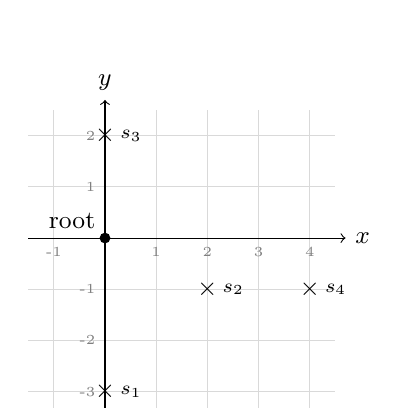
\begin{tikzpicture}[scale=0.65]
\draw[step=1, gray!30, thin] (-1.5,-3.5) grid (4.5,2.5);
\draw[->] (-1.5,0) -- (4.7,0) node[right, font=\small] {$x$};
\draw[->] (0,-3.5) -- (0,2.7) node[above, font=\small] {$y$};
\fill (0,0) circle (3pt) node[above left, font=\small] {root};
\foreach \x/\y/\l in {0/-3/s_1, 2/-1/s_2, 0/2/s_3, 4/-1/s_4} {
  \node[font=\small] at (\x,\y) {$\times$};
  \node[font=\scriptsize, right=2pt] at (\x,\y) {$\l$};
}
\foreach \x in {-1,1,2,3,4} \node[font=\tiny, gray, below] at (\x,0) {\x};
\foreach \y in {-3,-2,-1,1,2} \node[font=\tiny, gray, left] at (0,\y) {\y};
\end{tikzpicture}
\end{center}

\begin{enumerate}[label=(\alph*)]

\Needspace{4.0cm}
\item For each iteration, give the nearest existing node and the new node.

\begin{studentanswer}{2.6cm}
%%%%% SOLUTION HERE %%%%%
\end{studentanswer}

\clearpage
\textbf{P5 (continued)}
\item Draw the final tree on the coordinate grid, label the new nodes, and indicate
the nearest neighbor selected at iteration 2. If using LaTeX, add a line
inside the provided \texttt{tikzpicture} with
\texttt{\detokenize{\draw (x1,y1) -- (x2,y2);}}, replacing the endpoint
coordinates with those of the edge.

\begin{studentanswer}{6cm}
%%%%% SOLUTION HERE %%%%%
\begin{center}
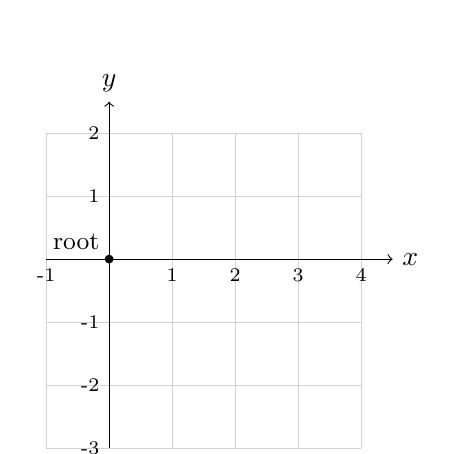
\begin{tikzpicture}[scale=0.8]
\draw[step=1,gray!35] (-1,-3) grid (4,2);
\draw[->] (-1,0)--(4.5,0) node[right] {$x$};
\draw[->] (0,-3)--(0,2.5) node[above] {$y$};
\fill (0,0) circle (2pt) node[above left,font=\small] {root};
\foreach \x in {-1,1,2,3,4} \node[below,font=\scriptsize] at (\x,0) {\x};
\foreach \y in {-3,-2,-1,1,2} \node[left,font=\scriptsize] at (0,\y) {\y};
\end{tikzpicture}
\end{center}
\end{studentanswer}

\Needspace{3.4cm}
\item Explain why the nearest node at iteration 2 is not the root. Support your answer with the relevant distances.

\begin{studentanswer}{2cm}
%%%%% SOLUTION HERE %%%%%
\end{studentanswer}

\end{enumerate}

\clearpage
\subsection*{P6 \gradstar Modified optimal heuristic}

Let $\heur^*(n)$ denote the optimal cost from cell $n$ to the goal on a
finite unit-cost grid. Assume every free cell can reach the goal. For a
fixed positive integer $k$, define
\[
\heur_k(n)=\max\bigl(\heur^*(n)-k,\,0\bigr).
\]
You may use without proof that $\heur^*$ is admissible and consistent.
Every edge has cost 1, and A* tests for the goal when removing a node
from the frontier.

\begin{enumerate}[label=(\alph*)]

\Needspace{3.9cm}
\item State the definitions of admissibility and consistency.

\begin{studentanswer}{2.5cm}
%%%%% SOLUTION HERE %%%%%
\end{studentanswer}

\Needspace{4.4cm}
\item Prove that $\heur_k$ is admissible for every fixed $k>0$.

\begin{studentanswer}{3cm}
%%%%% SOLUTION HERE %%%%%
\end{studentanswer}

\clearpage
\Needspace{5.4cm}
\item Prove that $\heur_k$ is consistent. Consider the cases $\heur^*(n)\leq k$ and $\heur^*(n)>k$ separately.

\begin{studentanswer}{4cm}
%%%%% SOLUTION HERE %%%%%
\end{studentanswer}

\Needspace{4.4cm}
\item Using parts (b) and (c), determine whether A* tree search and A* graph search with a closed set and no reopening return optimal paths under $\heur_k$. Identify the sufficient property for each guarantee.

\begin{studentanswer}{3cm}
%%%%% SOLUTION HERE %%%%%
\end{studentanswer}

\Needspace{4.4cm}
\item If $k\geq\max_n\heur^*(n)$, what algorithm does A* become? State whether it remains optimal and explain the effect on search effort.

\begin{studentanswer}{3cm}
%%%%% SOLUTION HERE %%%%%
\end{studentanswer}

\end{enumerate}

\clearpage
\section{Part 2: Programming}

In this part, you will complete selected steps of three planning methods
and compare their behavior on the supplied maps. These instructions are
self-contained: you do not need results from Part 1 to implement or run
the code. The provided programs load the maps, call your functions,
measure their behavior, and generate the plots. Your responsibility is
to complete the labeled TODO blocks and interpret the resulting output.

\paragraph{Before you begin.}
Use the course Python environment from PS0. Pull the course repository
to obtain this assignment, activate that environment, and open a terminal
in the repository root, the folder containing \texttt{sim/},
\texttt{ps0/}, and \texttt{ps1/}. All commands in this section are run
from that folder. If you need to recreate the environment, follow the
installation instructions in the repository's root \texttt{README.md}.
These experiments save images to files; they do not open an interactive
driving window.

\paragraph{What to edit.}
Your submission consists of four files in \texttt{ps1/code/}:
\begin{itemize}
\item \texttt{astar.py}: complete TODO A, which updates the search when
a cheaper route to a neighboring cell is found.
\item \texttt{vi.py}: complete TODO V, the value update for one state,
and TODO P, the greedy action choice for one state.
\item \texttt{policy\_iteration.py}: complete TODO I by reusing your
greedy action-selection function. The remaining policy-iteration code is provided.
\item \texttt{rrt.py}: complete TODO N, nearest-node selection, and
TODO E, a call to the provided steering function.
\end{itemize}
Replace each corresponding \texttt{raise NotImplementedError(...)} with
your implementation. Keep the function names, arguments, and return
formats unchanged. The surrounding scaffold is provided; you are not
expected to rewrite it. Read its comments to understand how your result
is used. Files described as provided are not part of your submission and
will be supplied by the grader.

\paragraph{How the programs fit together.}
The following paths are relative to \texttt{ps1/code/}. A runner is the
program you execute; it imports and calls the functions you complete.
\begin{center}\small
\begin{tabular}{p{0.20\linewidth}p{0.34\linewidth}p{0.35\linewidth}}
\textbf{Runner} & \textbf{Functions it calls} & \textbf{Provided support} \\\hline
\texttt{run\_astar.py} & \texttt{astar} in \texttt{astar.py} &
Map loading, \texttt{search\_utils.py}, result plots. \\
\texttt{compare.py} & \texttt{value\_iteration}, \texttt{extract\_policy},
\texttt{policy\_iteration}, and \texttt{astar} &
\texttt{grid\_mdp.py}, fixed-policy evaluation, timing and plots. \\
\texttt{run\_rrt.py} & \texttt{rrt} in \texttt{rrt.py} &
\texttt{dubins.py}, sampling, car motions, collision checks and plots.
\end{tabular}
\end{center}
Sections labeled \emph{Provided scaffold and interface} explain supplied
code; they are not implementation requirements. Only the TODOs require edits.

\clearpage
\subsubsection*{Suggested workflow and submission}
Work through Tasks 1, 2, and 3 in order. For each task, complete its TODOs,
run its public tests, and then run its experiment command. Task 2's
comparison also calls your A* implementation, so complete Task 1 first.
Task 3 does not depend on either of the other implementations.

The commands below run only the tests for the task you are working on:
\begin{lstlisting}
# Task 1
python -m pytest ps1/code/tests/test_astar.py -q
# Task 2
python -m pytest ps1/code/tests/test_vi.py -q
python -m pytest ps1/code/tests/test_policy_iteration.py -q
# Task 3
python -m pytest ps1/code/tests/test_rrt.py -q
\end{lstlisting}
An unfinished TODO raises \texttt{NotImplementedError}; this is expected
before you implement it. After completing a task, its tests should pass.
If a test fails, read the function name and assertion in the failure
report, then compare your implementation with the task's input and output
contract. Public tests cover small cases; passing them does not replace
running the supplied map experiments. Staff tests also exercise additional
cases. Do not change the tests to make an implementation pass.

Once all three tasks are complete, run the full public suite:
\begin{lstlisting}
python ps1/code/autograder.py
\end{lstlisting}
\paragraph{The complete coding report.}
Submit only two figures (the A* maze overlay and the RRT narrow plot),
one three-row A*/VI/PI comparison table for maze, and the three short
responses requested below, one per task. No other tables or plots are
required. Run all three maps to check your implementations; the extra
images and arrays are for your own inspection.

The experiment commands in the following pages save all requested images
in \texttt{ps1/figures/}. Open those files to inspect your results.
Fill the supplied comparison table in your PDF, or insert a legible
screenshot of the three maze rows. Use your own
measured results, including timing measurements from your machine.
The runners already produce the figures; you do not need to write
plotting code.

\paragraph{What to submit.}
Upload \texttt{astar.py}, \texttt{vi.py},
\texttt{policy\_iteration.py}, and \texttt{rrt.py} as the code submission.
Include the tables, images, and short explanations requested after each
task in your written-work PDF. Do not paste your Python implementations
into that PDF. Do not submit the simulator, helper files, tests, or saved
\texttt{.npy} arrays. If you use the editable TeX handout, insert each
figure and explanation in its corresponding \texttt{studentanswer}
environment. For example:
\begin{lstlisting}
\includegraphics[width=0.9\linewidth]
  {ps1/figures/ps1_astar_maze.png}
\end{lstlisting}

\clearpage

\subsection{Task 1: A* on occupancy grids}

\begin{quote}\small
\textbf{Task checklist.} Open \texttt{ps1/code/astar.py} and complete
TODO A. Run \texttt{test\_astar.py} using the command in the workflow
section, then run \texttt{run\_astar.py} as shown below. Submit the maze
overlay and a one- or two-sentence comparison of open and maze.
\end{quote}

\paragraph{Goal and inputs.}
A* finds a minimum-cost path from a specified start cell to a goal cell.
The runner loads each map, accounts for the robot's footprint, and calls
\texttt{astar(occ, start, goal, heuristic=manhattan)}. You receive
\texttt{occ}, a two-dimensional Boolean NumPy array, and two tuples
\texttt{start} and \texttt{goal}. A tuple is \texttt{(row, column)};
row zero is at the top and column zero is at the left.
\texttt{occ[row, column]} is \texttt{True} for an obstacle and
\texttt{False} for a free cell. The robot moves north, south, east, or
west, with cost 1 per move. There are no diagonal moves. You do not need
to convert world coordinates or load an image inside your function.

A* orders discovered cells by $f(n)=g(n)+h(n)$, where $g(n)$ is the
best cost found so far from the start and $h(n)$ estimates the remaining
cost to the goal. The supplied default is Manhattan distance,
$h(n)=|r_n-r_g|+|c_n-c_g|$, in grid moves. Always call the
\texttt{heuristic(cell, goal)} argument rather than hard-coding this
formula; the tests also use other heuristic functions.

\paragraph{Provided scaffold and interface.}
\texttt{search\_utils.py} provides \texttt{DeterministicFrontier},
\texttt{manhattan}, and the \texttt{SearchResult} return type.
\texttt{frontier.push(f, h, cell)} adds an entry;
\texttt{frontier.pop()} removes the smallest entry and returns
\texttt{(f, h, cell)}. The frontier orders entries by
$(f,h,\text{row},\text{column})$, with smaller values first.
Thus you do not implement a priority queue or tie-breaking rule.

The starter initializes \texttt{g} (best discovered costs),
\texttt{parent} (predecessors), \texttt{closed} (expanded cells), and
\texttt{expanded} (expansion order). It also supplies the search loop,
filters invalid neighbors, skips obsolete frontier entries, tests for
the goal, and reconstructs the final path. Duplicate frontier entries
are allowed: when you find a cheaper route, push a new entry and let the
provided stale-entry check discard the old one later.

\paragraph{Your implementation: TODO A.}
The TODO runs once for each valid neighboring cell \texttt{nb} of the
currently expanded \texttt{cell}. Update its route cost and A* priority:
\begin{enumerate}
\item Compute the candidate cost of reaching \texttt{nb} through
\texttt{cell}. Add the unit edge cost to \texttt{g[cell]}.
\item Compare that cost with \texttt{g.get(nb, math.inf)}. A missing
dictionary entry represents an undiscovered cell with infinite cost.
\item Only if the candidate is strictly smaller, update \texttt{g[nb]},
record \texttt{cell} as \texttt{parent[nb]}, and compute
$h=\texttt{heuristic(nb, goal)}$. Push \texttt{nb} with priority
$f=\texttt{g[nb]}+h$ (cost so far plus estimated remaining cost),
passing $h$ separately for tie-breaking. Otherwise, leave the search
state unchanged.
\end{enumerate}
These updates determine which cell the next frontier pop selects and
which predecessor the provided path-recovery code follows.

\clearpage
\subsubsection*{Task 1: checking and running your implementation}

\paragraph{Output contract.}
The scaffold returns \texttt{SearchResult(path, cost, expanded)}. The path must
include both the start and the goal, and its cost is the number of moves.
The \texttt{expanded} list records cells in expansion order, including
the start and goal. An expansion occurs when a non-stale entry is
removed from the frontier. Skip entries superseded by a cheaper route
or belonging to an already expanded cell. If no path exists, return an
empty path, infinite cost, and the expansion sequence accumulated before
the frontier became empty. Test for the goal when removing a valid entry
from the frontier.

The autograder checks expansion order as well as path cost. The provided
scaffold enforces the expansion conventions; leave that code unchanged.
For a small sanity check, two adjacent free cells have path cost 1, and
the returned path includes both cells. If start and goal coincide, the
cost is zero and the path contains that one cell.

Run your implementation on the three maps:
\begin{lstlisting}
python ps1/code/run_astar.py --out-dir ps1/figures
\end{lstlisting}
The command prints the path cost in grid moves and the number of
expanded nodes for each map. Each grid move corresponds to 0.05 m.
It also saves a plot for each map showing the expanded cells and the
returned path. The files are \texttt{ps1/figures/ps1\_astar\_open.png},
\texttt{ps1\_astar\_maze.png}, and \texttt{ps1\_astar\_narrow.png}
in that same folder. No interactive window is expected. Inspect all
three, but include only the maze overlay in your PDF; no A* table is required.

\textbf{Code submission.} Submit your implementation in \texttt{astar.py}.

\clearpage
\Needspace{5\baselineskip}
\textbf{PDF responses.}
\begin{enumerate}[label=(\alph*)]

\Needspace{9.5cm}
\item Include the A* overlay for \texttt{maze}.

\begin{studentanswer}{8cm}
%%%%% SOLUTION HERE %%%%%
\end{studentanswer}

\Needspace{4.5cm}
\item In one or two sentences, report the expansion counts on \texttt{open} and \texttt{maze} and explain how obstacles affect the usefulness of the Manhattan heuristic. No separate table is needed.

\begin{studentanswer}{3cm}
%%%%% SOLUTION HERE %%%%%
\end{studentanswer}

\end{enumerate}
\clearpage
\subsection{Task 2: Value iteration and policy iteration}

\begin{quote}\small
\textbf{Task checklist.} Complete TODOs V and P in \texttt{vi.py}, then
TODO I in \texttt{policy\_iteration.py}. Run \texttt{test\_vi.py} and
\texttt{test\_policy\_iteration.py}, then \texttt{compare.py}.
Task 1 must work before this comparison can run. Submit only the maze
comparison table and a two- or three-sentence interpretation; no plot is required.
\end{quote}

\paragraph{Goal and model.}
Compute a value and a preferred action for every free cell using value
iteration (VI) and policy iteration (PI). A value is the predicted
discounted return from a cell; a policy specifies the action to take
there. The runner constructs a \texttt{GridMDP} using cells of width
1.0 m. Both methods use the known
transition and reward model; neither learns from sampled experience.
Actions are north, south, east, and west. An attempted move into a wall
or beyond the boundary leaves the robot in place. Entering the goal
gives reward $+10$ and ends the episode; other transitions give zero.
The terminal value is zero and $\gamma=0.9$. Your functions must use
their supplied \texttt{gamma} argument rather than hard-coding 0.9.

\paragraph{The world interface.}
Your functions receive a \texttt{world} object. You need only these
members; map loading and transitions are already implemented:
\begin{itemize}
\item \texttt{world.shape} is \texttt{(number of rows, number of columns)}.
\item \texttt{world.free\_cells()} returns the free-cell tuples, including the goal.
\item \texttt{world.goal} is the terminal \texttt{(row, column)} tuple.
\item \texttt{world.step(s, a)} returns \texttt{(s2, reward, done)}:
the successor cell, immediate reward, and a Boolean indicating termination.
Actions are integer indices: 0 is north, 1 south, 2 east, and 3 west.
Pass an index, not a direction vector.
\end{itemize}
A value array \texttt{V} has shape \texttt{world.shape}; \texttt{V[s]}
accesses the value at tuple \texttt{s}. Walls contain \texttt{NaN}, and
the goal contains zero. A policy array has the same shape but contains
integer action indices; walls and the goal contain $-1$.

\paragraph{Your implementation: TODO V in \texttt{vi.py}.}
The scaffold supplies initialization, the sweep and state loops, and
the convergence test for
\texttt{value\_iteration(world, gamma, tol, max\_sweeps)}.
For each free nonterminal state $s$, compute the four one-step returns
\[
b_a=\begin{cases}
r, & \text{if \texttt{world.step(s,a)} reports termination},\\
r+\gamma V_k(s'), & \text{otherwise},
\end{cases}
\qquad V_{k+1}(s)=\max_{a\in\{0,1,2,3\}} b_a.
\]
Call \texttt{world.step} to obtain $s'$ and $r$ for each action.
Write the maximum into \texttt{V\_new[s]}. Read successor values from
\texttt{V}, the previous sweep, not \texttt{V\_new}; this is synchronous
value iteration. The scaffold initializes all free cells to zero,
retains zero at the goal, and leaves walls as \texttt{NaN}.
It stops after the first sweep whose largest absolute value change is
below \texttt{tol}, or after \texttt{max\_sweeps}. It returns
\texttt{(V, sweeps\_run)}, counting the final sweep. You do not implement
the stopping or counting logic.

\clearpage
\subsubsection*{Task 2: extracting and improving a policy}
\paragraph{Your implementation: TODO P in \texttt{vi.py}.}
\texttt{extract\_policy(world, V, gamma)} receives a value table and
returns a greedy action grid. For each free nonterminal state, evaluate
the same four one-step returns as in TODO V. Store the \emph{index of
the maximizing action} in \texttt{policy[s]}, not the maximum value.
Evaluate actions in order 0, 1, 2, 3. In a tie, select the smaller
action index; \texttt{np.argmax} on an action-ordered list gives this
rule. Do not change the supplied \texttt{V}. Initialization and the state
loop are provided, including the $-1$ entries for walls and the goal.

\paragraph{Your implementation: TODO I in \texttt{policy\_iteration.py}.}
The supplied PI loop starts with an all-north policy on nonterminal
states. It alternates evaluating that fixed policy and improving it,
stopping when the action grid no longer changes. The provided
\texttt{evaluate\_policy} function solves the fixed-policy equations;
you do not need to implement or modify its linear algebra.

Your \texttt{improve\_policy(world, V, gamma)} receives the values of
the \emph{current} policy and should return actions greedy with respect
to that table. This is exactly the operation in \texttt{extract\_policy}.
Reuse that function: a one-line call returning its result is sufficient
and intended. Do not run value iteration here, since that would replace
evaluation of the current policy with a different computation.

\paragraph{How the runner uses your functions.}
\texttt{compare.py} constructs the world, calls your
\texttt{value\_iteration}, and passes its returned table to your
\texttt{extract\_policy}. It then calls the provided
\texttt{policy\_iteration} loop, which repeatedly calls
\texttt{evaluate\_policy} and your \texttt{improve\_policy}.
Finally, it calls your A* function for the fine-grid comparison.
Complete Task 1 before running this full comparison.

\paragraph{Check and run.}
Use the two Task 2 test commands listed at the start of Part 2. As a
sanity check, an action entering the goal has one-step return 10,
not $10+\gamma\cdot10$: the goal has no future return. Then run:
\begin{lstlisting}
python ps1/code/compare.py --plot-dir ps1/figures
\end{lstlisting}

The runner reports path length and
planning time for each method, together with A* expansion counts, VI
sweep counts, and PI evaluation/improvement rounds. These counts measure
different operations: a PI round includes a policy-evaluation solve.
Compare measured times as well as counts; do not infer a speedup from
the number of rounds alone. The runner checks agreement between the
two MDP value tables and saves \texttt{ps1/figures/ps1\_values.png} and
\texttt{ps1/code/out/values\_\{open,maze,narrow\}.npy}.
The arrays and value plot are for inspection, not submission. A failed value-table
comparison is an error to investigate, not a result to include in your
table. A* uses 0.05 m cells and VI/PI use 1.0 m cells; compare distances
in meters, not raw numbers of steps.

\textbf{Code submission.} Submit \texttt{vi.py} and
\texttt{policy\_iteration.py}. The provided helper and loop should remain unchanged.

\clearpage
\paragraph{What the comparison can tell you.}
VI and PI use the same states, transitions, reward, and goal, so their
values should agree. Their timing comparison concerns these two
implementations on your machine. A* uses a finer grid and answers a
single start-to-goal query rather than computing a policy for all states;
its timing is contextual, not a controlled test of which algorithm is
universally faster. RRT also imposes car-motion constraints and uses a
different maze endpoint, so it is not part of this timing comparison.

\textbf{PDF responses.}
\begin{enumerate}[label=(\alph*)]
\item \begin{minipage}[t]{\linewidth}
Fill the table below using only the three \texttt{maze} rows printed by
\texttt{compare.py}. Keep the work-count units: expansions for A*, sweeps
for VI, and rounds for PI. You may fill the supplied table or replace it
with a legible screenshot of those three rows.

\begin{studentanswer}{5cm}
%%%%% SOLUTION HERE %%%%%
\begin{center}\small
\renewcommand{\arraystretch}{1.7}
\begin{tabular}{l|c|c|c}
Method & Path (m) & Work count (with unit) & Time (ms) \\\hline
A* & & & \\
VI & & & \\
PI & & &
\end{tabular}
\end{center}
\end{studentanswer}

\end{minipage}
\item \begin{minipage}[t]{\linewidth}
In two or three sentences, identify whether VI or PI was faster on your
machine and explain why comparing sweep and round counts alone would
not establish that result. Give one reason the A* timing is not a
like-for-like comparison with these two methods.

\begin{studentanswer}{4cm}
%%%%% SOLUTION HERE %%%%%
\end{studentanswer}

\end{minipage}
\end{enumerate}

\clearpage
\subsection{Task 3: RRT with car motion constraints}

\begin{quote}\small
\textbf{Task checklist.} Open \texttt{ps1/code/rrt.py} and complete
TODOs N and E. Run \texttt{test\_rrt.py}, then \texttt{run\_rrt.py}.
Submit the narrow plot and a two- or three-sentence explanation of the
least efficient map's sample-to-node ratio. No results table is required.
\end{quote}

\paragraph{Goal and representation.}
A rapidly exploring random tree (RRT) grows a tree of feasible car
motions from the start toward sampled states. Unlike the grid planners,
it represents a state as a NumPy array \texttt{[x, y, theta]} in meters,
meters, and radians. The car cannot turn in place or move sideways.
The supplied steering function accounts for its turning constraint;
you implement neither car dynamics nor a steering solver.

The runner builds a \texttt{DubinsWorld}, creates a seeded random
generator, and calls
\texttt{rrt(world, start, goal, rng, step, goal\_bias, goal\_tol, max\_iters)}.
The tree is a list of pairs \texttt{(state, parent\_index)} in insertion
order. Its root is \texttt{(start, -1)}. For example,
\texttt{tree[i][0]} is node $i$'s state, and \texttt{tree[i][1]} is
the index of its predecessor. An index identifies a node in this list;
it is not a grid coordinate.

\paragraph{Provided scaffold and interface.}
The starter supplies the loop, 5\% goal-biased sampling, node insertion,
collision rejection, goal test, counters, and path recovery. Each
iteration first decides whether to sample the goal; otherwise it calls
\texttt{world.sample\_free(rng)} to obtain a free state. Leave these
random draws unchanged so runs with the same seed are reproducible.
You need these two provided calls:
\begin{itemize}
\item \texttt{dubins\_steer(world, state, target, step)} tries three
forward motions of arc length \texttt{step}: maximum left steering,
straight, and maximum right steering. It discards colliding arcs and
returns the feasible endpoint closest to the target's $(x,y)$ position,
or \texttt{None} if all three motions are blocked. The endpoint need
not reach the target. The target's orientation does not affect selection.
\item \texttt{world.collision\_free(state)} reports whether the car's
collision footprint at that state is free. The scaffold uses this as
an additional endpoint check after steering.
\end{itemize}

\paragraph{Your implementation: TODO N.}
For the current \texttt{sample}, find the nearest node already in
\texttt{tree} by scanning \texttt{enumerate(tree)}. Compare squared
Euclidean distances $(x_i-x_s)^2+(y_i-y_s)^2$, ignoring orientation.
Update \texttt{nearest\_i} and \texttt{nearest\_d2} only when the new
distance is strictly smaller. Thus the earliest inserted node wins
an exact tie. Do not reorder the tree: its parent indices depend on
that order. No spatial-search library is needed.

\paragraph{Your implementation: TODO E.}
Call \texttt{dubins\_steer} with \texttt{world}, the selected node's
state \texttt{tree[nearest\_i][0]}, \texttt{sample}, and \texttt{step}.
Assign the returned endpoint (or \texttt{None}) to \texttt{new}. This
TODO is a single function call. The supplied code then either rejects
the extension or inserts \texttt{new} with parent \texttt{nearest\_i}.

\clearpage
\subsubsection*{Task 3: checking and running your implementation}
\paragraph{Output contract and stopping.}
The scaffold returns an \texttt{RRTResult} with four fields:
\texttt{path}, \texttt{tree}, \texttt{samples\_drawn}, and \texttt{nodes\_added}.
It tests the goal only after adding a new node. Success means that node's
$(x,y)$ distance from the goal is strictly less than \texttt{goal\_tol};
the final orientation is not constrained. The returned path includes
the start and the successful endpoint. If the iteration budget is
exhausted, \texttt{path} is \texttt{None}, but the tree and counters
are still returned. \texttt{samples\_drawn} counts every loop iteration,
including rejected extensions and goal samples; \texttt{nodes\_added}
counts accepted extensions, excluding the root. A useful check is
\texttt{len(tree) == nodes\_added + 1}.

The runner supplies a motion length of 0.3 m, goal-sampling probability
0.05, goal tolerance 0.5 m, budget 8000 iterations, and random seed 26.
These settings are already in \texttt{constants.py}; do not change them
or hard-code them into your function. On \texttt{maze}, the car's goal
is the supplied checkpoint $(13.5,7.5)$ below the map's goal chamber.
The chamber entrance does not admit the car with this task's clearance.
Use the \texttt{goal} argument exactly as supplied, rather than replacing
it with the grid planners' goal.

\paragraph{Check and run.}
After completing both TODOs, run the Task 3 public tests, then:
\begin{lstlisting}
python ps1/code/run_rrt.py --plot-dir ps1/figures
\end{lstlisting}
For each map, the command
reports the number of samples drawn and the number of nodes added by
collision-free extensions. It also plots the tree and returned path.
All images are saved in \texttt{ps1/figures/}:
\texttt{ps1\_rrt\_open.png}, \texttt{ps1\_rrt\_maze.png}, and
\texttt{ps1\_rrt.png} for narrow. Only the narrow image is required in
your PDF. The optional \texttt{--save-artifacts} flag is not needed.
The last printed column is \emph{nodes per sample}; the response below
asks for \emph{samples per added node}, which you should compute from
the two count columns.

\begin{center}
\includegraphics[width=0.45\linewidth]{ps1/figures/rrt_dubins_example.pdf}
\captionof{figure}{An RRT on the \texttt{open} map. Each edge follows a
motion primitive that satisfies the car's turning constraint.}
\end{center}

\textbf{Code submission.} Submit your implementation in \texttt{rrt.py}.

\Needspace{5\baselineskip}
\textbf{PDF responses.}
\begin{enumerate}[label=(\alph*)]

\Needspace{9.5cm}
\item Include \texttt{ps1\_rrt.png}, showing the tree and highlighted path on \texttt{narrow}.

\begin{studentanswer}{8cm}
%%%%% SOLUTION HERE %%%%%
\end{studentanswer}

\Needspace{5.0cm}
\item Identify the map with the largest ratio of samples drawn to nodes added and state that ratio. Explain in two or three sentences how the map geometry and motion constraints contribute to it. No separate table is needed.

\begin{studentanswer}{3.5cm}
%%%%% SOLUTION HERE %%%%%
\end{studentanswer}

\end{enumerate}

\docfooter
\end{document}
